\vspace{35mm}
\begin{figure}[h!]\centering
\captionsetup{width=\textwidth}
\caption{Pumping Cost Externality: Densities for San Joaqu\'{i}n Valley}
\label{fig:dwl_densities}
\vspace{-2mm}
{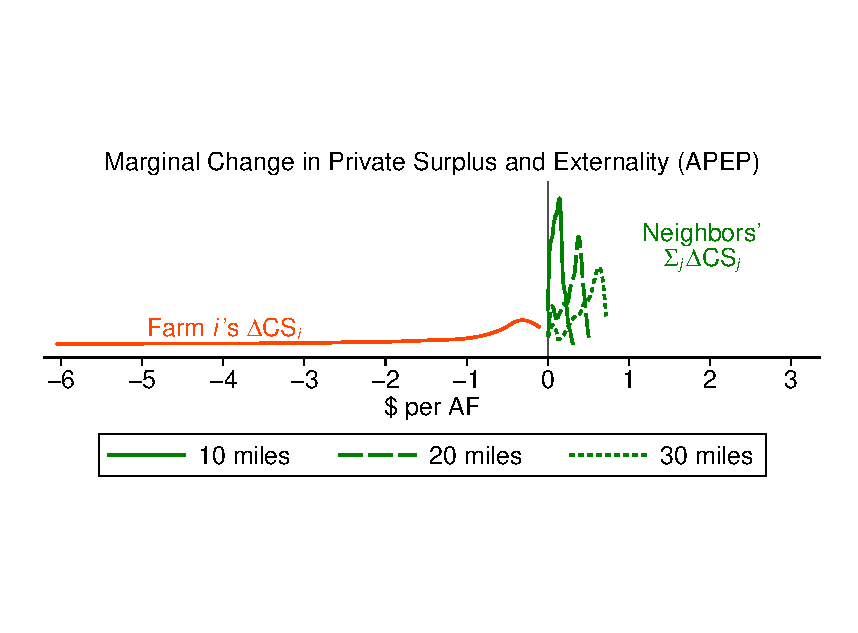
\includegraphics[trim={0 22mm 0 21mm}, clip, width=.84\textwidth]{figures/ext_dcs_j.eps}}\\
\vspace{2mm}
{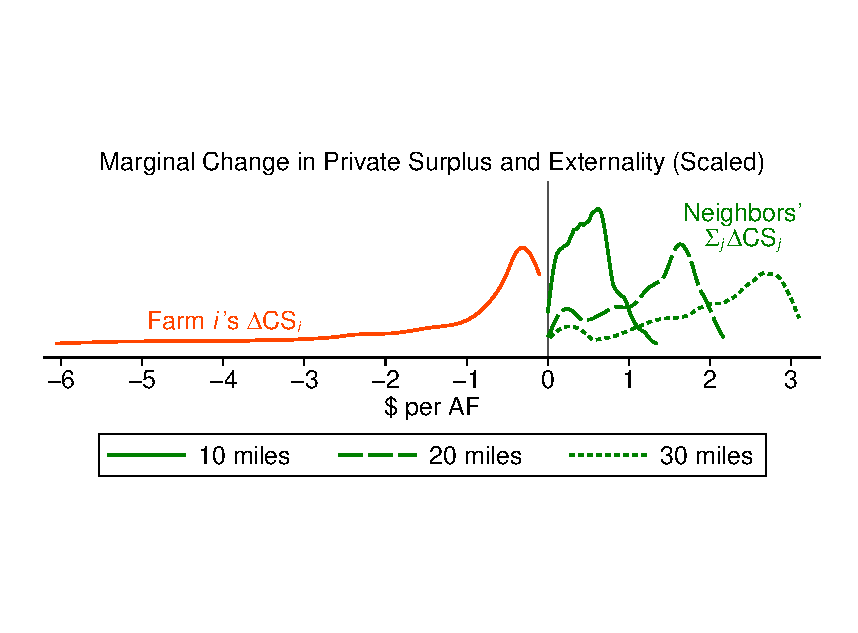
\includegraphics[trim={0 22mm 0 18mm}, clip, width=.84\textwidth]{figures/ext_dcs_j_scaled.eps}}\\
\vspace{2mm}
{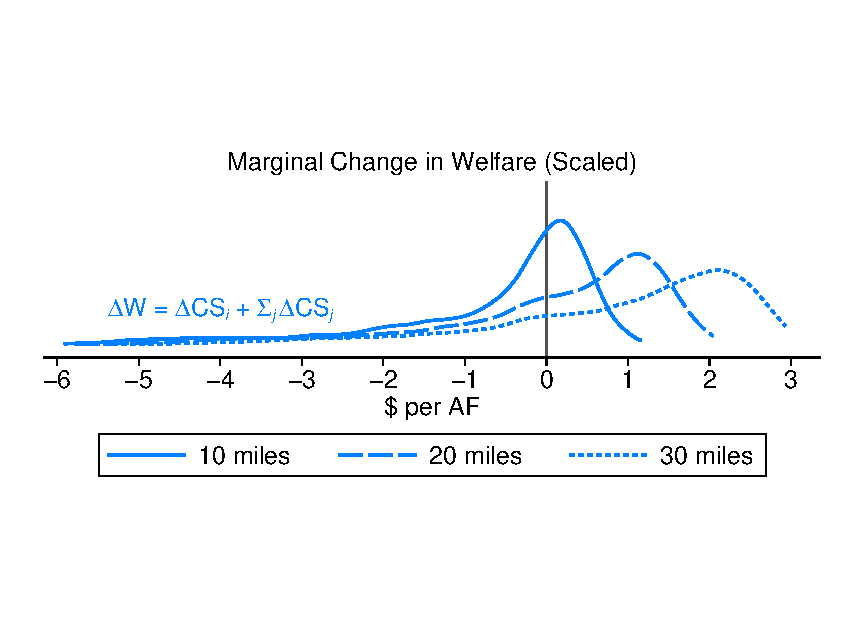
\includegraphics[trim={0 22mm 0 18mm}, clip, width=.84\textwidth]{figures/ext_dw_scaled.eps}}\\
\vspace{2mm}
\captionsetup{width=\textwidth}
\caption*{\footnotesize \emph{Notes:} This figure plots kernel densities for marginal changes in surplus, for APEP farms in the San Joaqu\'{i}n Valley (as reported in the righthand columns of Table \ref{tab:externality_calcs}). Red densities show the distribution of farm $i$'s change in private surplus from pumping 1 AF less in June 2016. Green densities show distributions of surplus gains for farm $i$'s neighbors (within $r$-mile circles) in July 2016, which are not reported in Table \ref{tab:externality_calcs}. Blue densities sum the orange and green densities to show the net change in welfare (as in the bottom 3 panels of Table \ref{tab:externality_calcs}); positive mass indicates deadweight loss, where farm $i$'s marginal pumping cost externality is larger than its marginal private surplus.  The middle and bottom densities scale up our APEP-matched sample to include unmatched agricultural electricity consumers likely to be groundwater pumpers. All densities omit farms outside the 10th-to-90th percentiles of $\Delta CS_i$, for ease or presentation. See text for further details.
}
\end{figure}